\documentclass[../Main.tex]{subfiles}

\begin{document}
\author{Interference} %use author for title of lesson
\date{Year 1 Topic 18} %use date to refer to topic in main booklet

\section{Interference} %Section is the title of the lesson repeated, ready for the main contents page.

\begin{frame}{Phase Difference - recap}
Consider the two waves below. They are identical, but there is a phase difference between them - what is this phase difference in radians?
\begin{figure}
    \centering
    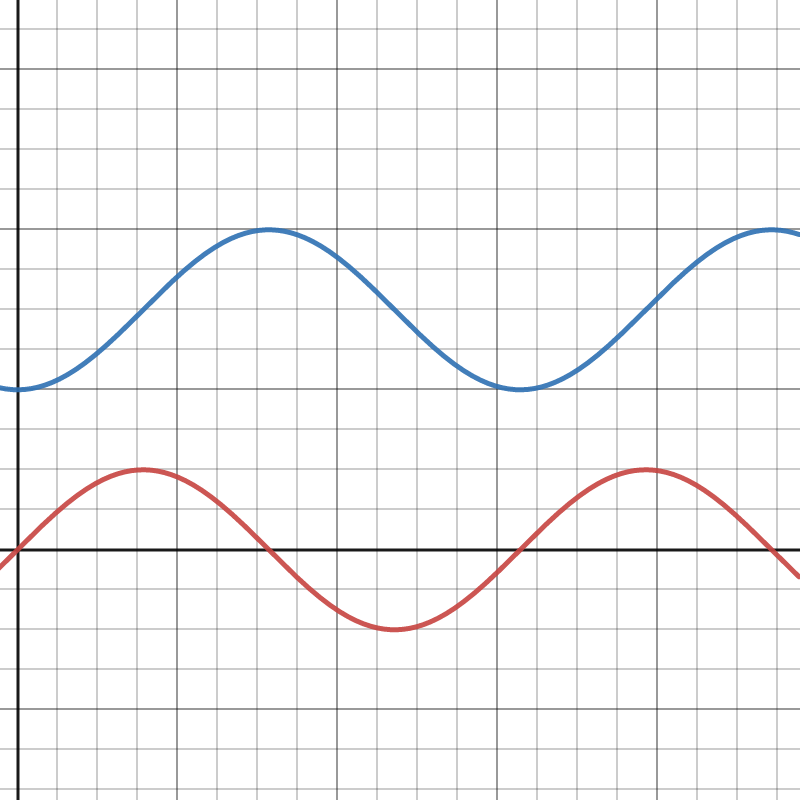
\includegraphics[width=5cm]{Waves_Images/wavesoutofphase.png}
\end{figure} \pause
\begin{equation*}
    \phi = \frac{\pi}{2}
\end{equation*}
Keep this in mind, as we will be seeing this later...
\end{frame}

\begin{frame}{Superposition}
    If two waves overlap in space, they will interact with each other. The principle of superposition says that their displacements sum to create a single wave. When this happens, the waves are said to \emph{superpose}.
    
    \begin{block}{More formally...}
    The principle of superposition states that when two waves meet at a point, the resultant displacement at that point is equal to the sum of the displacements of the original wave.
    \end{block}
    
    This has some interesting results, and works better for exactly identical waves as we shall see shortly...
\end{frame}

\begin{frame}{Interference}
     The waves are said to interfere with each other -- this is true for all waves, longitudinal and transverse. There are two types of interference, \emph{constructive} and \emph{destructive}.
    \pause
    \begin{multicols}{2}
    Constructive interference is when two waves are exactly in phase -- their displacements add together.
    \pause
    \columnbreak

    Destructive interference is when two waves are exactly out of phase -- their displacements subtract from each other.
    \end{multicols}
    
    \begin{figure}
        \centering
        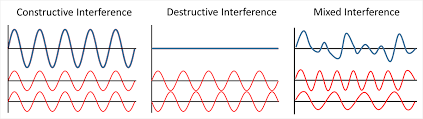
\includegraphics[width=0.8\textwidth]{Waves_Images/interference.png}
    \end{figure}
\end{frame}

\begin{frame}{Coherent waves}
    \begin{block}{Coherent waves}
    Coherent waves are two waves that are emitted from different sources that have a constant phase difference. Hence, they must also have the same frequency. 
    \end{block}
    \begin{figure}
        \centering
        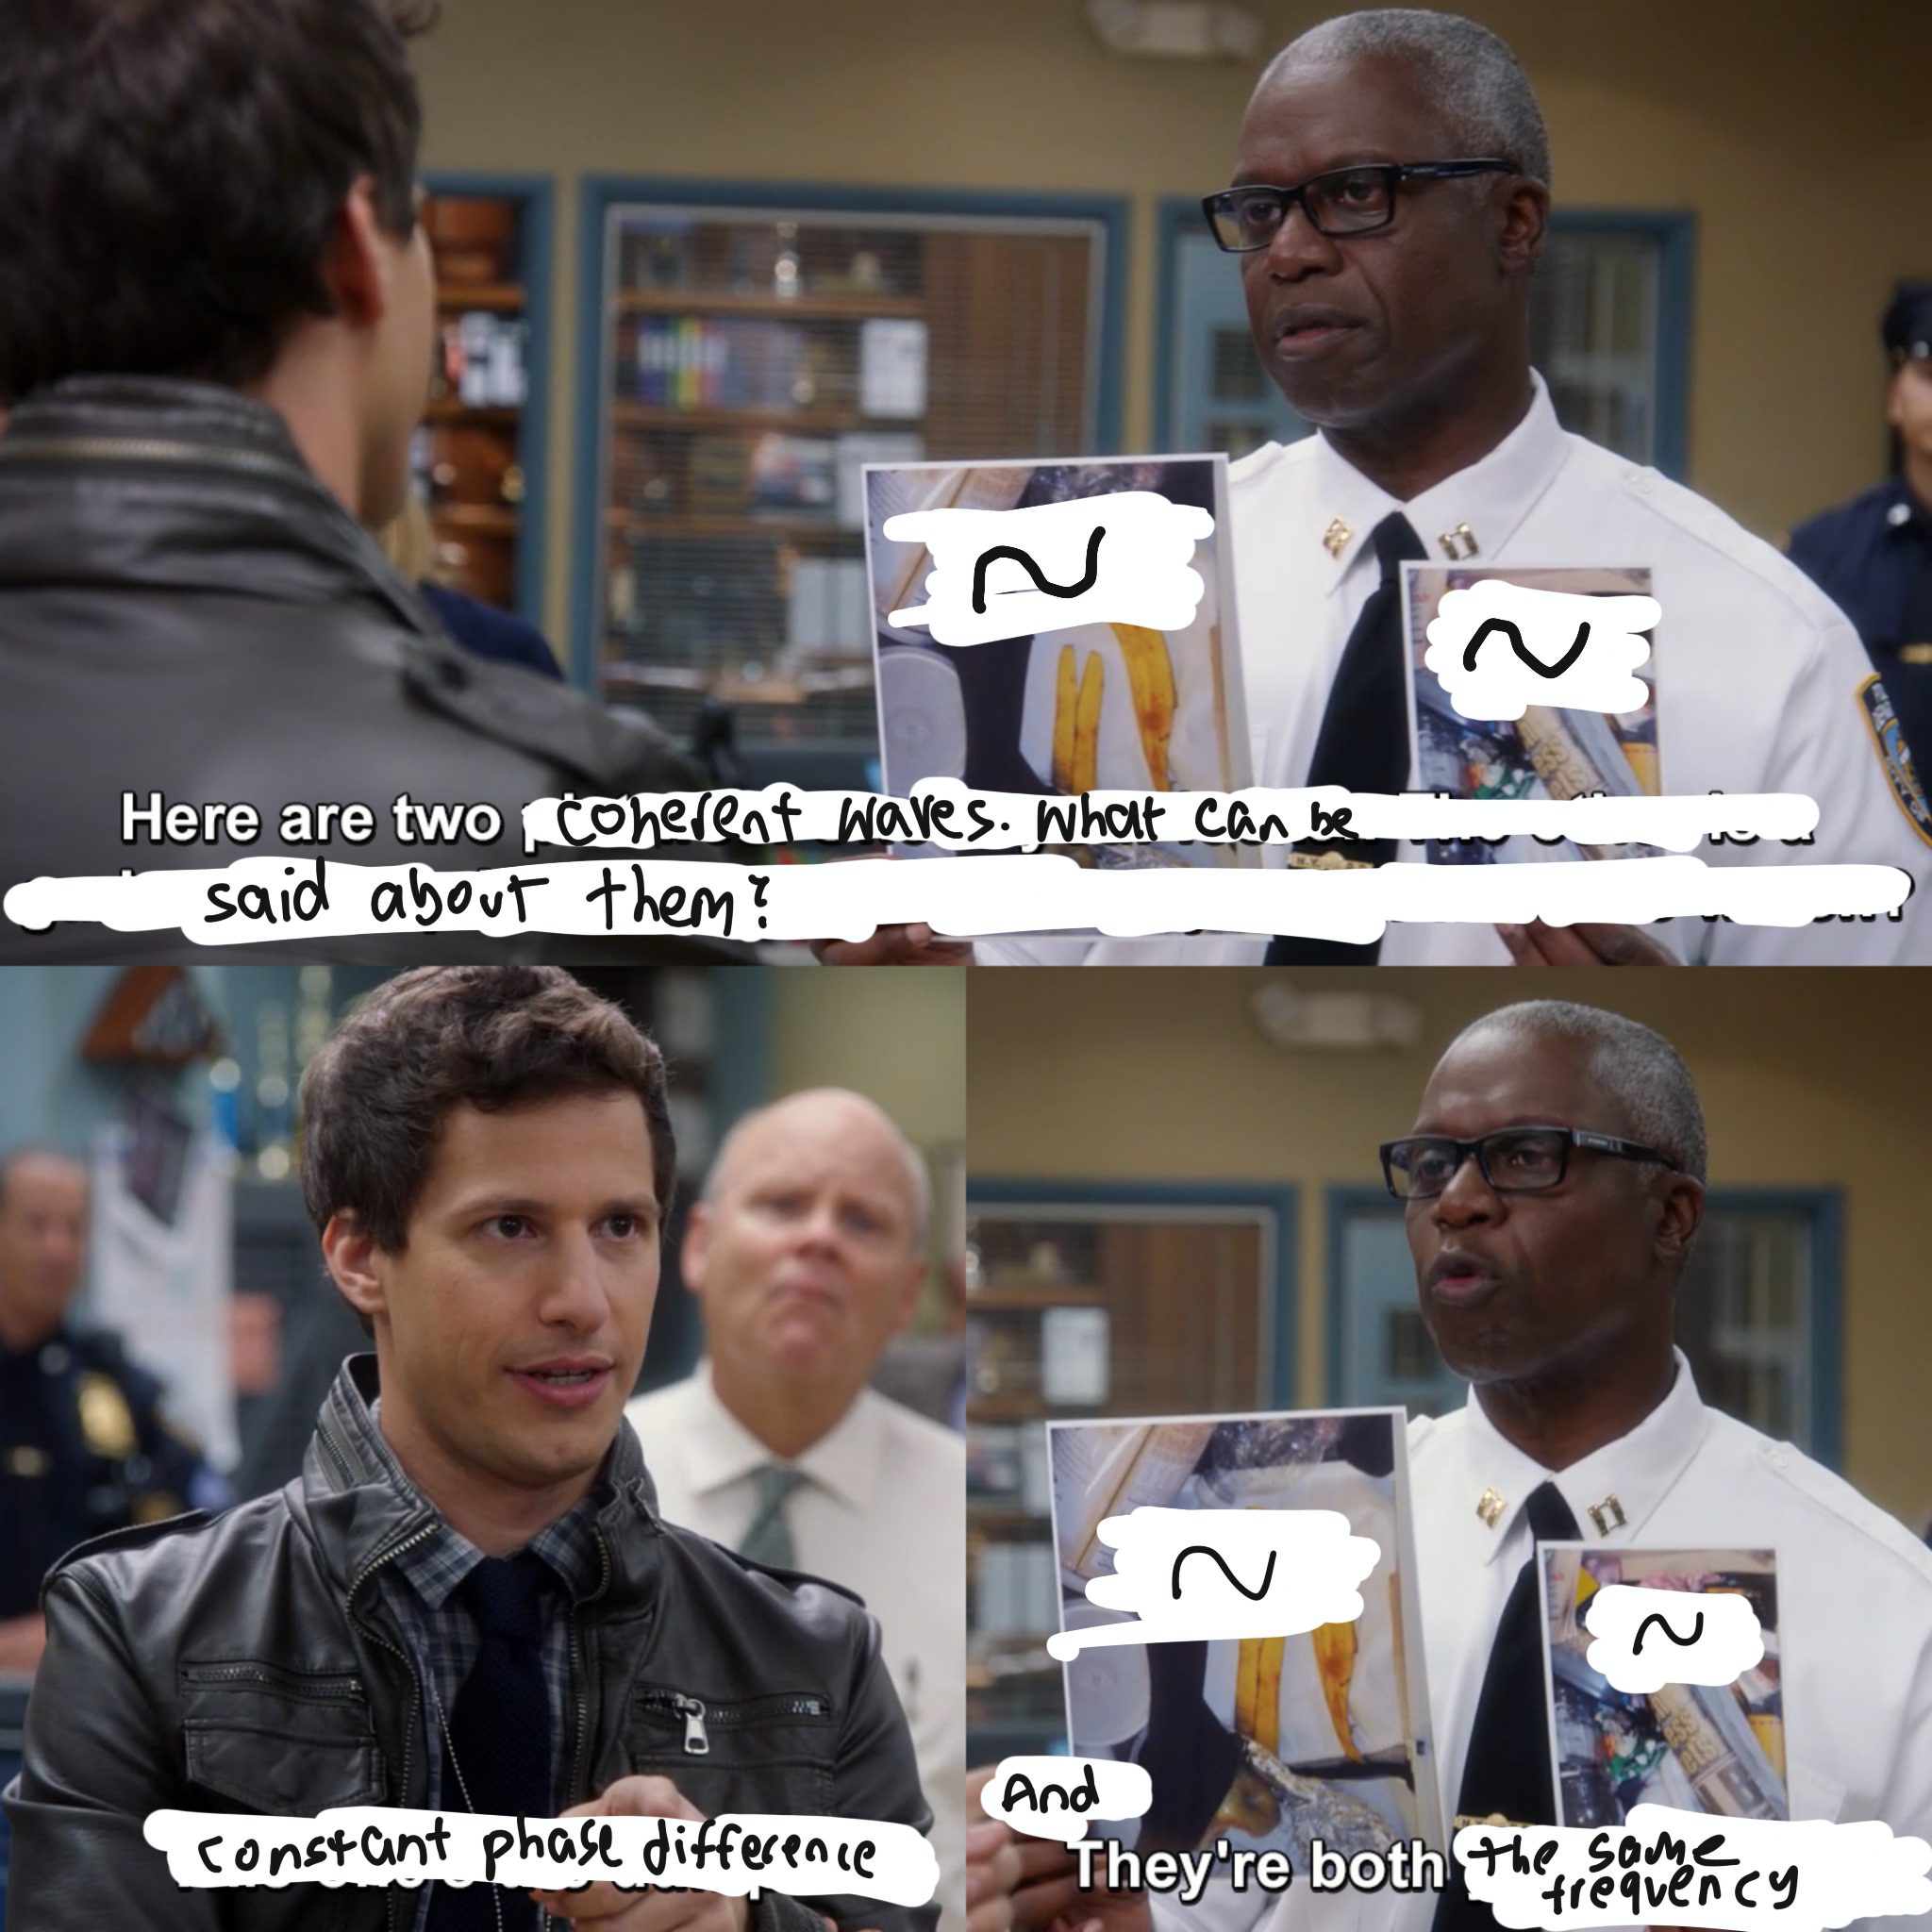
\includegraphics[width=4cm]{Waves_Images/coherentwavesmeme.png}
    \end{figure}
    The waves from the first slide are coherent - they have the same frequency and a constant phase difference.
\end{frame}

\begin{frame}{Sources of sound}
Two speakers connected to the same output will produce two coherent waves. Since sound spreads out, we will see regions of constructive and destructive interference where we arrive at points in and out of phase.
    \begin{figure}
        \centering
        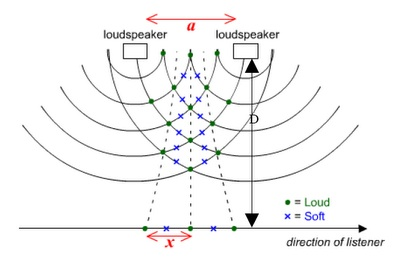
\includegraphics[height=4cm]{Waves_Images/interferenceofsound.jpg}
    \end{figure}
    Walking in a straight line parallel to the line connecting the speakers at any perpendicular distance will result in alternating points of constructive and destructive interference, known as maxima and minima. 
\end{frame}

\begin{frame}{Path Difference}
    In order to constructively interfere, we must have a phase shift of $2n\pi$ radians, for any integer n. This must mean that we are $n\lambda$ apart, so the physical difference in distance travelled from two sources must also be $n\lambda$. 
    
    \begin{block}{Path Difference}
    The physical difference in distance travelled by two coherent waves from source to detector.
    \end{block}
    \pause
    
    Looking at the geometry, there will always be a point exactly between the speakers to form an isosceles triangle that is the exact same distance between the two speakers. This will always be a maximum, as there is no path difference. 
    \newline
    \pause
    \newline
    If we travel across we will find the next maxima will be at n=1, then n=2, etc. These adjacent maxima will be at some distance x apart, a distance that can be calculated (as we shall see on Monday)
\end{frame}

\begin{frame}{Path Difference}
    \begin{figure}
        \centering
        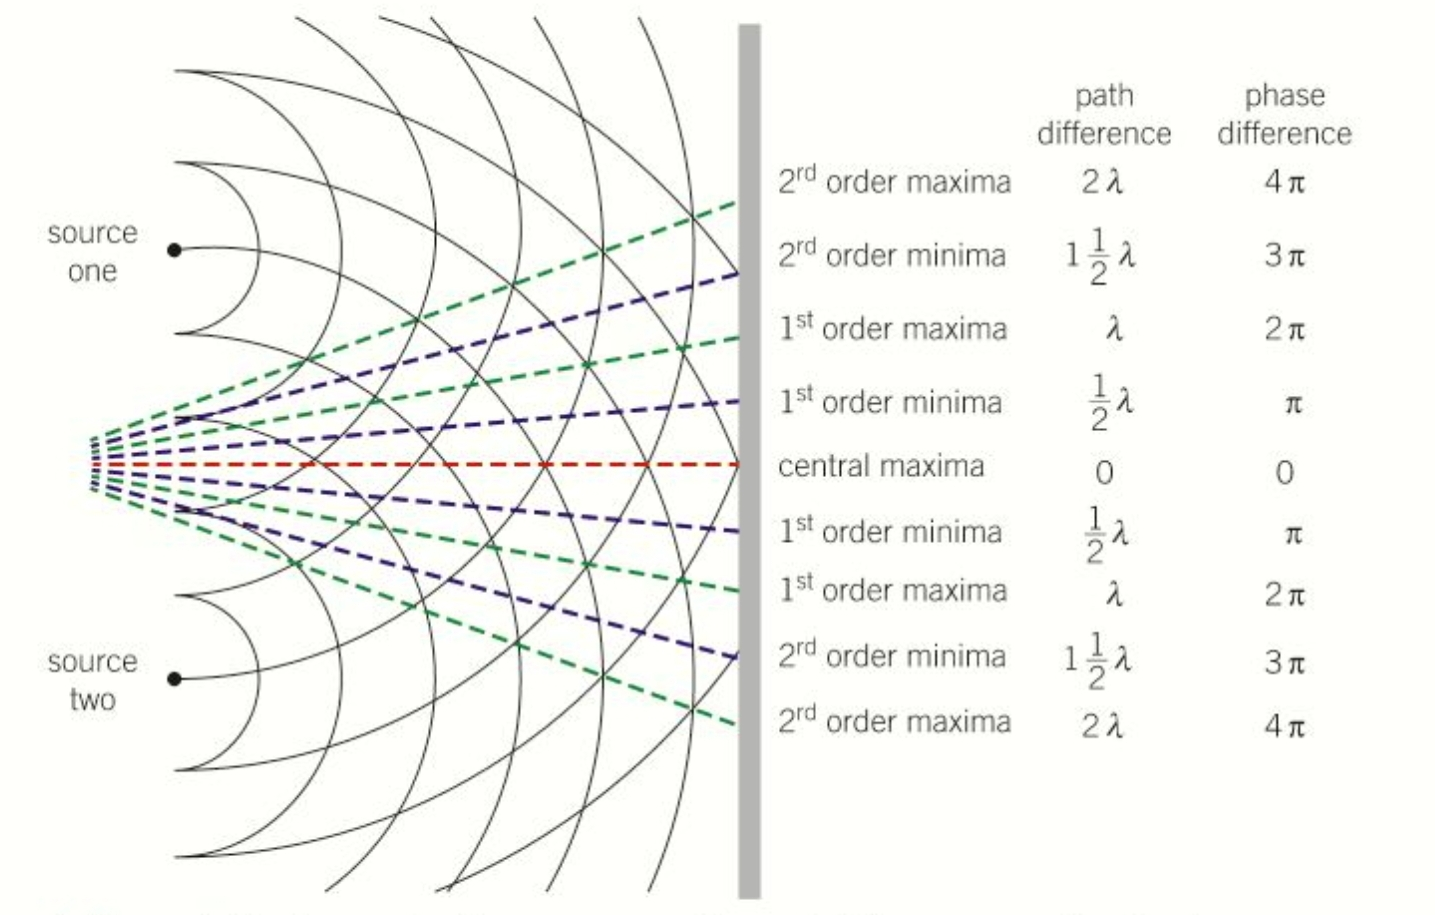
\includegraphics[width=0.9\textwidth]{Waves_Images/pathdifference.jpg}
    \end{figure}
\end{frame}

\end{document}